\subthesischapter{Pruebas del sistema}

% SUBSECTION 3.2: WORK FLOW
\subsubthesischapter{Descripción de un flujo de trabajo}
A continuación, se muestra el flujo normal, asociado a la ejecución de una rutina de entrenamiento de juego serio, partiendo del estado en el que el sistema no está iniciado (este flujo de trabajo, teóricamente, sería el más utilizado una vez implementado el sistema):

\begin{figure}[ht]
    \centering
    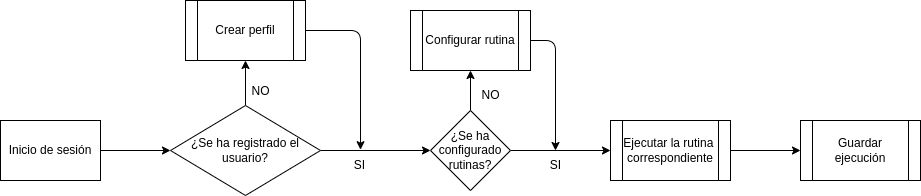
\includegraphics[scale=0.5]{images/diagram-flow.png}
    \caption{Flujo normal asociado a una rutina de entrenamiento}
    \label{fig: diagram-flow}
\end{figure}

Para iniciar el proceso, el usuario debe ingresar sus credenciales en la interfaz de Inicio de Sesión, como se muestra en el anexo 2(a). En caso de que el usuario no tenga una cuenta registrada en el sistema, será redirigido automáticamente a la interfaz de registro, anexo 2(b). En este paso, se le permitirá crear un nuevo usuario para poder acceder al sistema. Tras iniciar sesión, se despliega la interfaz principal, brindando al usuario la capacidad de realizar diversas acciones, tales como configurar y dar inicio a un proceso de entrenamiento anexo 3a anexo 3b, iniciar el proceso de calibración anexo 3(c), examinar estadísticas relevantes anexo 5 y revisar o editar la información detallada en su perfil anexo 4(a) y 4(b) así como elegir una rutina ya configurada anexo 4(c).

\vspace{5pt}
Si la rutina de entrenamiento deseada no se encuentra disponible, el usuario tiene la posibilidad de interactuar directamente con la aplicación accediendo a la interfaz de configuración de parámetros correspondiente a la modalidad que desea establecer. En el caso de la modalidad Ligero, anexo 3(a), se le solicita al usuario ingresar manualmente los valores de distancia o tiempo, específicos al nivel de dificultad del entrenamiento que busca. Por otro lado, en la modalidad Clínico anexo 3(b) y 3(c), la interacción se intensifica, ya que el usuario debe calibrar el sistema para obtener los valores esenciales de línea base y MCV. A partir de este último valor, el usuario asume un papel activo al elegir el porcentaje que se asignará a la rutina de rehabilitación por canal, basándose en criterios médicos. Una vez que se han establecido estos parámetros, el usuario continúa su interacción con la aplicación al ingresando los valores específicos de distancia o tiempo correspondiente a la rutina de entrenamiento Clínico. 

\vspace{5pt}
Al hacer clic en el botón \underline{Comenzar}, se presenta la escena de juego correspondiente. Al finalizar, los resultados obtenidos son almacenados en la base de datos y pueden ser visualizados en la sección de estadísticas de la interfaz. 

% SUBSECTION 3.2: FUNCTIONAL REQUIREMENTS
\subsubthesischapter{Comprobación de los requisitos funcionales del sistema}
La comprobación de los requisitos funcionales del sistema, mostrada en la tabla \ref{tab: darkbox1}, se realizó a partir de una prueba de caja negra. Dicha prueba puede definirse como una técnica donde se busca la verificación de las funcionalidades del software o aplicación analizada, sin tomar como referente la estructura del código interno, las rutas de tipo internas ni la información referente a la implementación. Esto quiere decir que se llevan a cabo con desconocimiento del funcionamiento del sistema interno, debido a que se enfoca en la entrada y salida de un software, tomando como base sus especificaciones y requisitos.    

\begin{table}[h]
    \centering
    \begin{tabularx}{\textwidth}{|c|X|X|X|}
        \hline
        \textbf{No} & \textbf{Entrada} & \textbf{Respuesta esperada} & \textbf{Respuesta esperada}\\\hline
        % 1
        1
        &
        \begin{minipage}{0.3\columnwidth}
            \textbf{campo correo} (cadena de caracteres asociada con un correo registrado en la base de datos). \\\\ \textbf{campo contraseña} (la contraseña correspondiente al correo registrado).
        \end{minipage}  
        & 
        Permite al usuario acceder al sistema. 
        & 
        Se accede al sistema correctamente.
        \\\hline
        
        % 2
        2
        &
        \begin{minipage}{0.3\columnwidth}
            \textbf{campo correo} (cadena de caracteres que no posea formato de correo). \\\\ \textbf{campo contraseña} (Cualquier cadena de caracteres).
        \end{minipage}  
        & 
        El sistema notifica con el mensaje: Correo inválido.
        & 
        Se notifica correctamente el mensaje: Correo inválido. (ver anexo 1(a))
        \\\hline

        % 3
        3
        &
        \begin{minipage}{0.3\columnwidth}
            \textbf{campo correo} (cadena de caracteres asociada con un correo registrado en la base de datos). \\\\ \textbf{campo contraseña} (Contraseña distinta a la correspondiente con el correo registrado).
        \end{minipage}  
        & 
        El sistema notifica con el mensaje: Contraseña incorrecta.
        & 
        Se notifica correctamente el mensaje: Contraseña incorrecta. (ver anexo 1(c))
        \\\hline
        % 4
        4
        &
        \begin{minipage}{0.3\columnwidth}
            \textbf{campo correo} (cadena de caracteres asociada con un correo que no esté registrado en la base de datos). \\\\ \textbf{campo contraseña} (Contraseña distinta a la correspondiente con el correo registrado).
        \end{minipage}  
        & 
        El sistema notifica con el mensaje: Correo incorrecta.
        & 
        \cellcolor{red!75} Error
        \\\hline

    \end{tabularx}
    \caption{Prueba de caja negra, inicio de sesión}
    \label{tab: darkbox1}
\end{table}

La prueba de caja negra para la funcionalidad de inicio de sesión se llevó a cabo mediante la implementación de varios casos de prueba, cada uno de los cuales involucraba múltiples iteraciones para abordar distintas combinaciones de entradas. Estas iteraciones se realizaron con el objetivo de evaluar exhaustivamente el comportamiento del sistema en diversas situaciones. En el caso 4 se evidenció un error, para su solución se realizó una revisión del código fuente para determinar la causa subyacente. Luego, se implementó medidas correctivas, como son, ajustes en el código y en la lógica de manejo de errores, con el objetivo de resolver y evitar futuros incidentes similares.

% SUBSECTION 3.2
\subsubthesischapter{Encuesta a especialistas sobre la percepción del sistema}
Fue aplicada una encuesta a 10 profesionales del área de la investigación 4 de ellos doctores en ciencia, 3 ingenieros entre ellos 1 informático, 1 ingeniero de control automático y 1 bio-médico especialistas en desarrollo en el tema de la rehabilitación y 3 especialistas del área médica. Todos con más de 5 años de experiencia.

\vspace{5pt}
Los resultados de la encuesta a los profesionales en cuanto a los requisitos no funcionales (usabilidad e interoperabilidad) además de los evaluados por \cite{franco2016sistema} (ergonomía, seguridad y concordancia de los ejercicios con los de la terapia tradicional) se presentan agrupados en una escala dicotómica en la Tabla \ref{table:test}.

\begin{table}[ht]
    \centering
    \begin{tabular}{p{3cm} c c c c}
        \hline
        Característica      &  Alto(\#/Total)   &  Alto(\%) & Bajo(\#/Total)  & Bajo(\%) \\\hline
        Usabilidad          &  7/10   &  70   & 3/10  &   30\\
        Interoperabilidad   &  8/10   &  80   & 2/10  &   20\\
        Ergonomía           &  10/10  &  100  & 0/10  &   0\\
        Concordancia        &  8/10   &  80   & 2/10  &   20\\
        Seguridad           &  10/10  &  100  & 0/10  &   0\\
        \hline        
    \end{tabular}        
    \caption{Resultados de percepción de los especialistas}
    \label{table:test}
\end{table}

Dichos resultados siguen el patrón lógico esperado:
\begin{itemize}
    \item \textbf{Usabilidad (70\% de satisfacción alta):} Un alto nivel de usabilidad significa que los profesionales evaluados encontraron el juego serio fácil de usar y comprender. Esto indica que la interfaz y las interacciones del juego son intuitivas, lo que facilita su adopción por parte de los usuarios.
    
    La facilidad de uso es fundamental para los pacientes de neurorehabilitación, especialmente para aquellos que pueden tener limitaciones cognitivas o motoras. Un juego fácil de entender y jugar fomenta la participación y la adherencia al programa de rehabilitación


    \item \textbf{Interoperabilidad (80\% de satisfacción alta):} Una alta interoperabilidad sugiere que el juego serio puede integrarse sin problemas con el sistema de adquisición de datos.
    
    La interoperabilidad es crucial en un entorno de neurorehabilitación donde se utilizan varios dispositivos y sistemas para monitorear y apoyar la recuperación del paciente. Un juego serio interoperable permite una recopilación de datos sin problemas y una comunicación eficaz entre diferentes componentes del sistema.


    \item \textbf{Ergonomía y Seguridad (100\% de satisfacción alta):}En el caso de la seguridad aplican condiciones similares a la ergonomía, dado que el sistema por sí mismo incluye las condiciones asociadas con una bicicleta estática que ya es usada en los procesos de rehabilitación de miembro inferior. Además la ergonomía también demuestra la capacidad de la aplicación para adaptarse a las necesidades y habilidades cambiantes del usuario. 
    
    La seguridad total indica que los profesionales evaluados consideran que el juego serio no representa ningún riesgo para la salud o la integridad de los usuarios.
    
    \item \textbf{Concordancia (80\% de satisfacción alta):} Implica que los ejercicios en el juego serio se alinean adecuadamente con las prácticas de terapia tradicional, lo que sugiere coherencia en el enfoque de rehabilitación. Los ejercicios en el juego deben complementar y respaldar las técnicas utilizadas en la terapia tradicional. 
    
    La concordancia asegura que los pacientes practiquen movimientos y habilidades relevantes para su recuperación.
\end{itemize}

Las observaciones generales proporcionadas por los especialistas, permitieron identificar otros potenciales usos en el proceso de rehabilitación de víctimas de ACV: resistencia, fuerza y coordinación,actividad física independiente de su condición, complemento al proceso de entrenamiento de marcha, coordinación, autoconfianza, motivación. Los hallazgos anteriores van de acuerdo con investigaciones preliminares donde se muestra que con el uso de bicicletas estáticas en rehabilitación se puede fortalecer a parte de dichas habilidades mencionadas la capacidad física, aeróbicas, además de comprobar un mejoramiento en el sistema cardiovascular y respiratorio del paciente \cite{phadke2019impact, nardone2017passive}.

\vspace{5pt}
Por otra parte, teniendo en cuenta que el sistema de adquisición de datos no es invasivo y, por el contrario, presentó aceptación por parte de los especialistas por incluir un videojuego, se propone, en un futuro, realizar pruebas a un número determinado de pacientes víctimas de ACV y de esta manera evaluar el funcionamiento del sistema de adquisición de datos durante ejercicios de rehabilitación resistida y activa-asistida, en los que el paciente moverá los pedales continuamente y realizará por su propia acción o con ayuda de especialista los ejercicios establecidos. Adicionalmente, se valida la hipótesis de que el sistema no es exclusivo para rehabilitación de personas víctimas de ACV, por lo tanto se plantea que en un trabajo futuro se podrá probar dicha aplicación en la modalidad ligero, por ejemplo, con deportistas de alto rendimiento con lesiones deportivas.

\vspace{5pt}
En gran medida la impresión positiva es porque el desarrollo se convierte en un reto para el usuario y una ayuda a la concentración en una actividad paralela de entretenimiento mientras realiza el proceso de rehabilitación. Si bien se recibieron comentarios  positivos otros también fueron negativos respecto a la usabilidad y la concordancia, requisitos estrechamente relacionados en el juego serio. En ambos se encontró como deficit el no cubrir toda la gamma de ejercicios definidos en las rutinas de rehabilitación siendo propuestos para futuras versiones la inclusión de las modalidades resistida y activo-asistida con el fin de complementar los ejercicios de rehabilitación que se pueden realizar actualmente con el sistema de adquisición de datos, los cuales son solamente ejercicios de rehabilitación libre.
